\documentclass[12pt, a4paper]{article}
\usepackage[a4paper, mag=1000, left=1.5cm, right=1.5cm, top=2cm, bottom=2cm, headsep=0.7cm, footskip=1cm]{geometry}
\usepackage[T2A]{fontenc}
\usepackage[utf8]{inputenc}
\usepackage[english,russian]{babel}
\usepackage[colorlinks=true, citecolor=blue, urlcolor=blue, linkcolor=blue]{hyperref}
\usepackage{graphicx}
\usepackage{physics}
\usepackage{amsmath,amssymb}
\usepackage{float}
\usepackage{titlesec}
\usepackage{ulem}
\usepackage{xcolor}
\usepackage{tcolorbox}

\definecolor{mypink}{RGB}{255, 230, 230}  % Светло-розовый фон
\definecolor{myred}{RGB}{153, 0, 51}  % Темно-красный для заголовка и полоски

% Оформление блока с полоской слева
\newtcolorbox{mybox}{
    colback=mypink,   % Фон внутри блока
    colframe=myred,   % Цвет левой полоски
    boxrule=4pt,      % Толщина полоски (шире = толще)
    left=10pt,        % Отступ текста от левой полоски
    right=5pt, top=5pt, bottom=5pt, % Отступы внутри блока
    enhanced,         % Улучшенное отображение
    sharp corners,    % Отключаем закругления
    frame hidden,     % Прячем рамку (кроме левой полоски)
}

\titleformat{\section}{\Large\bfseries\centering}{}{0em}{}
\renewcommand{\thesection}{}
\newcommand{\RomanNumeralCaps}[1]{\MakeUppercase{\romannumeral #1}}

\begin{document}
    \thispagestyle{empty}

% Оформление титульного листа
    \begin{center}
    {\Large\textbf{ФЕДЕРАЛЬНОЕ ГОСУДАРСТВЕННОЕ АВТОНОМНОЕ ОБРАЗОВАТЕЛЬНОЕ УЧРЕЖДЕНИЕ ВЫСШЕГО ОБРАЗОВАНИЯ}}
        \\
        {\Large\textbf{«НАЦИОНАЛЬНЫЙ ИССЛЕДОВАТЕЛЬСКИЙ УНИВЕРСИТЕТ ИТМО»}}\\[5mm]
        {\large\text{ФАКУЛЬТЕТ ТЕХНОЛОГИЙ ИСКУССТВЕННОГО ИНТЕЛЛЕКТА}}\\[5mm]
        
\includegraphics[scale=0.14]{logo.png}\\[30mm]
        \rule{\textwidth}{0.4mm}\\[3mm]
        {\Large\text{Индивидуальное домашнее задание}}\\[3mm]
        {\Large\text{по дисциплине “Математический анализ и основы вычислений”}}\\[3mm]
        {\Large\textf{Вариант № 33}}\\[3mm]
        \rule{\textwidth}{0.4mm}
    \end{center}

    \vfill

    \begin{flushright}
        \large Выполнил: \\
        Студент группы J3111 \\
        Воробьев Андрей Павлович \\
        ИСУ: 465440 \\
        Преподаватель: \\
        Табиева А.В. \\
    \end{flushright}

    \vfill

    \begin{center}
        \large Санкт-Петербург \\
        \large 2025
    \end{center}

    \newpage

    \titleformat{\section}{\Large\bfseries\raggedright}{}{0em}{}
    \titleformat{\subsection}{\large\bfseries\raggedright}{}{0em}{}

    \setlength{\parindent}{0pt}

\section*{Задание 1}
\textf{Исследовать данную функцию на равномерную непрерывность на данном мно жестве пользуясь определением.\\}
{\large
    \[
        f(x) = 2x - \sqrt{x} + \frac{1}{x - 1},\ a)X = [2, +\infty), \ b)X = (0, 1)
    \]
}
\textbf{\Large Решение:\\}

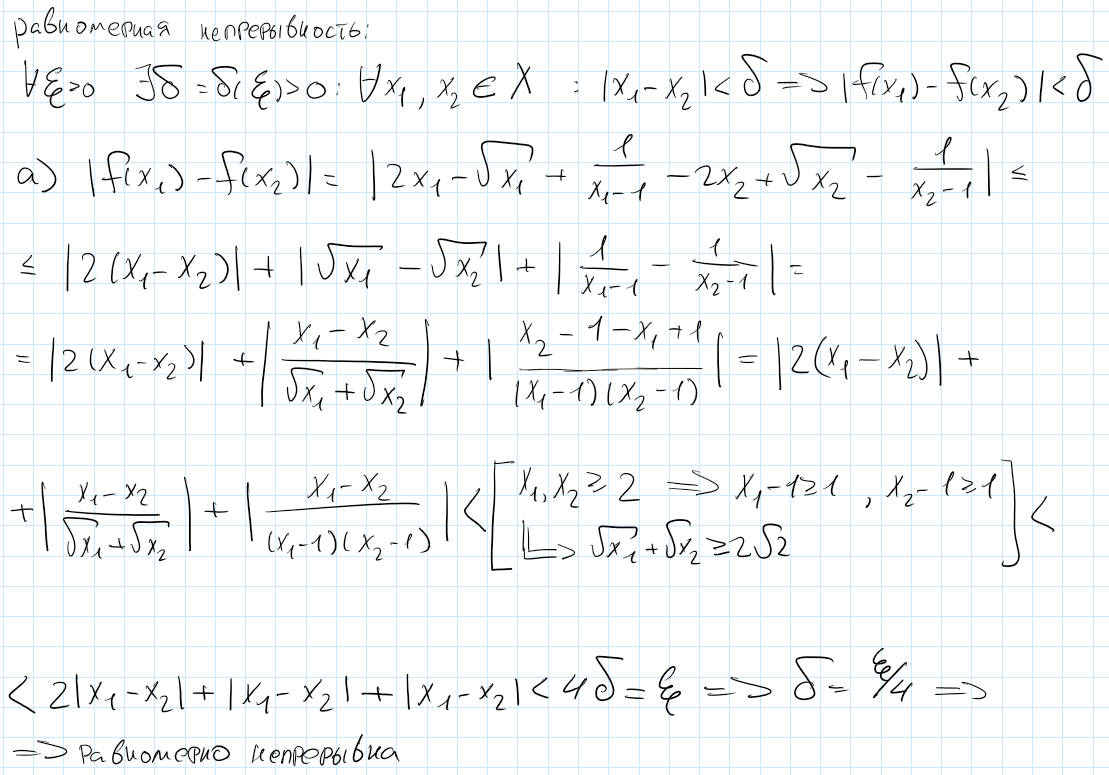
\includegraphics[width=\textwidth]{images/img11}
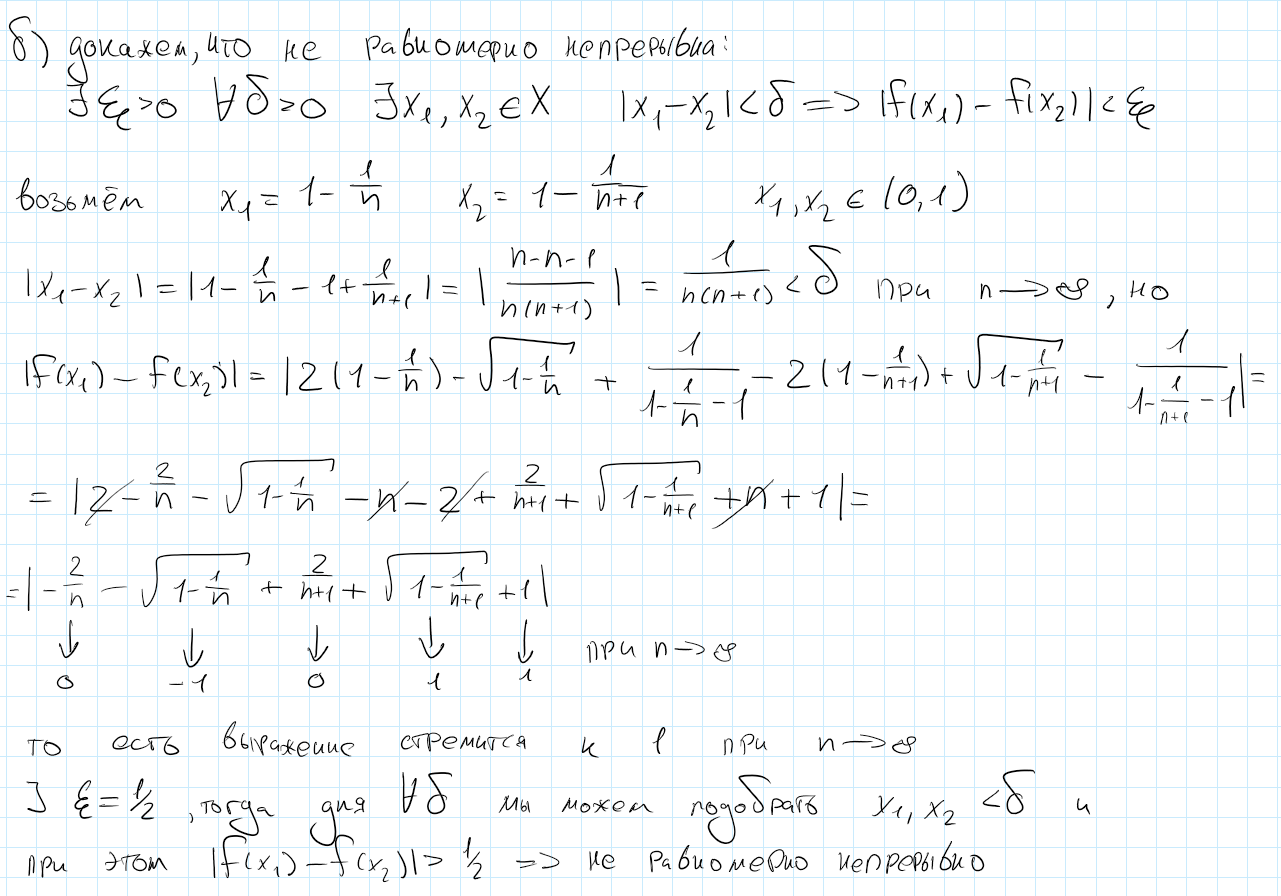
\includegraphics[width=\textwidth]{images/img12}
\newpage

\section*{Задание 2}
\textf{Преобразовать выражение к интегральной сумме, доказать существование соответствующего интеграла и найти предел.\\}
{\large
    \[
        \lim\limits_{n \to \infty} (\frac{n}{n^2 + 1} + \frac{n}{n^2 + 4} + \cdots + \frac{n}{n^2 + n^2})
    \]
}
\textbf{\Large Решение:\\}

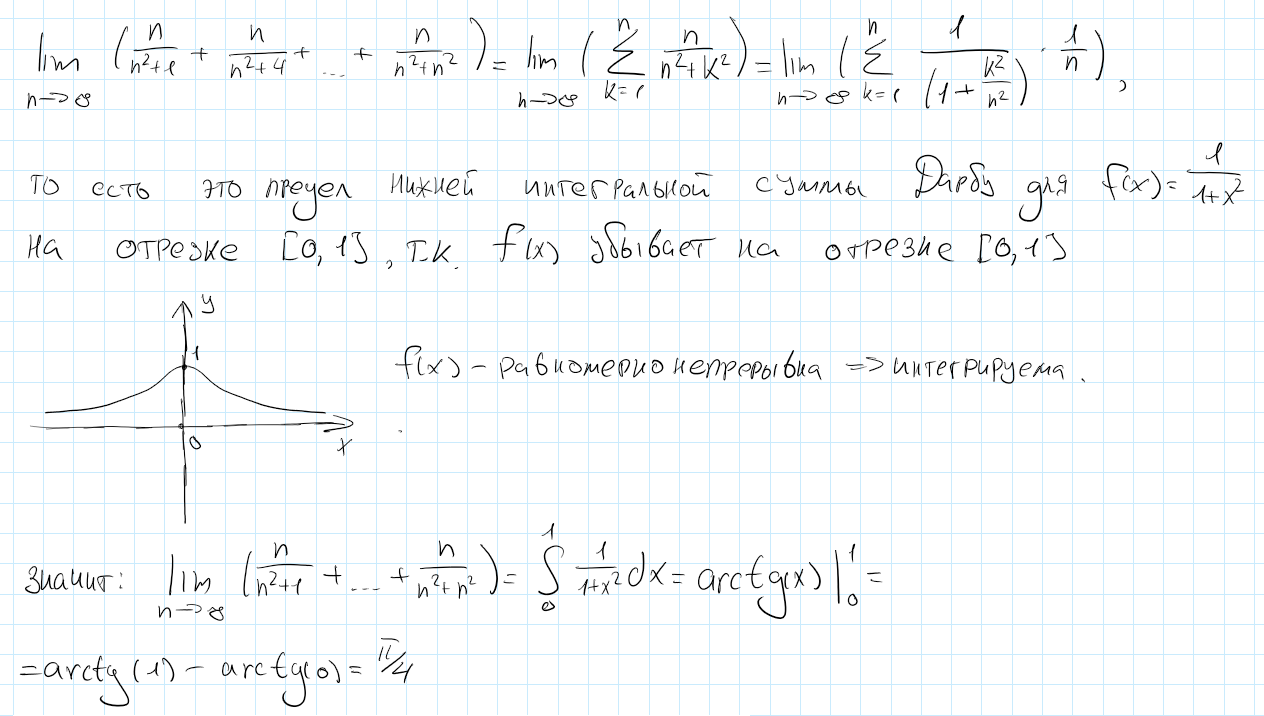
\includegraphics[width=\textwidth]{images/img21}
\newpage

\section*{Задание 3}
\textf{Найти площадь фигуры, ограниченной кривой, заданной параметрически. Сделать рисунок.}
{\large
    \[
        x = n\cos t - \cos(nt) \quad y = n\sin t - \sin(nt) \quad (n \in \mathbb{N})
    \]
}
\textbf{\Large Решение:\\}

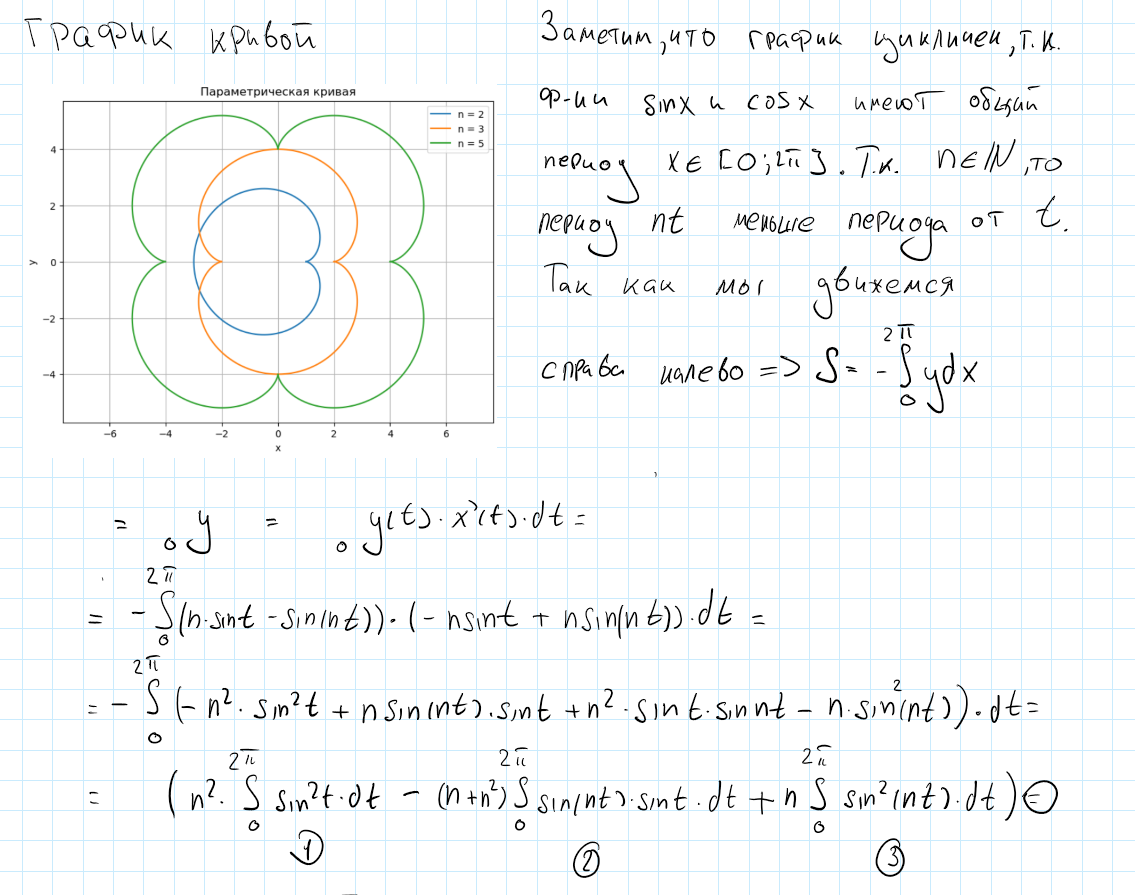
\includegraphics[width=\textwidth]{images/img31}
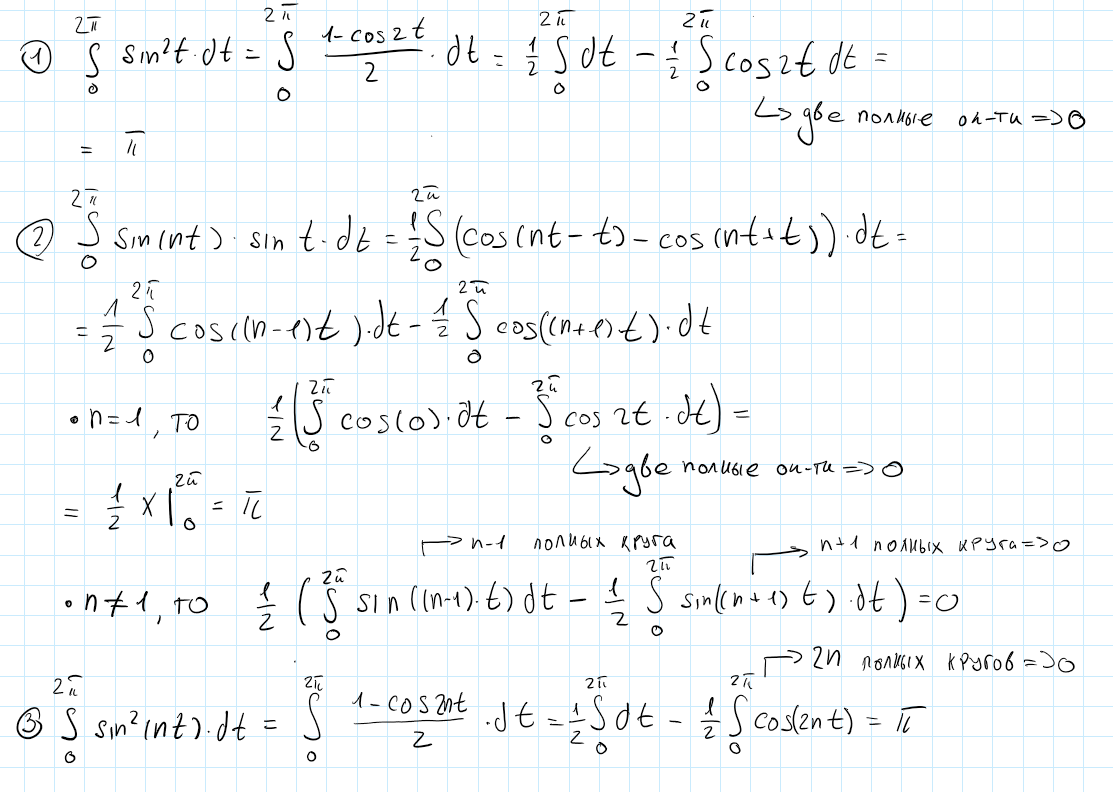
\includegraphics[width=\textwidth]{images/img32}
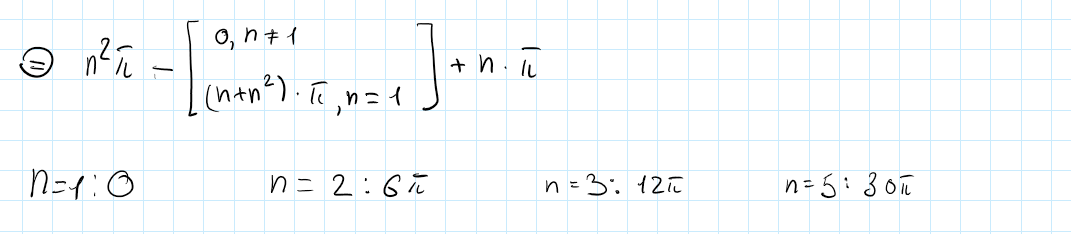
\includegraphics[width=\textwidth]{images/img33}
\newpage

\section*{Задание 4}
\textf{Кривая задана как пересечение поверхностей, заданных данными у равнениями в декартовых координатах. Задайте кривую параметрически и найдите длину кривой}
{\large
    \[
        x^6 + y^6 = a^2x^2y^2
    \]
}
\textbf{\Large Решение:\\}

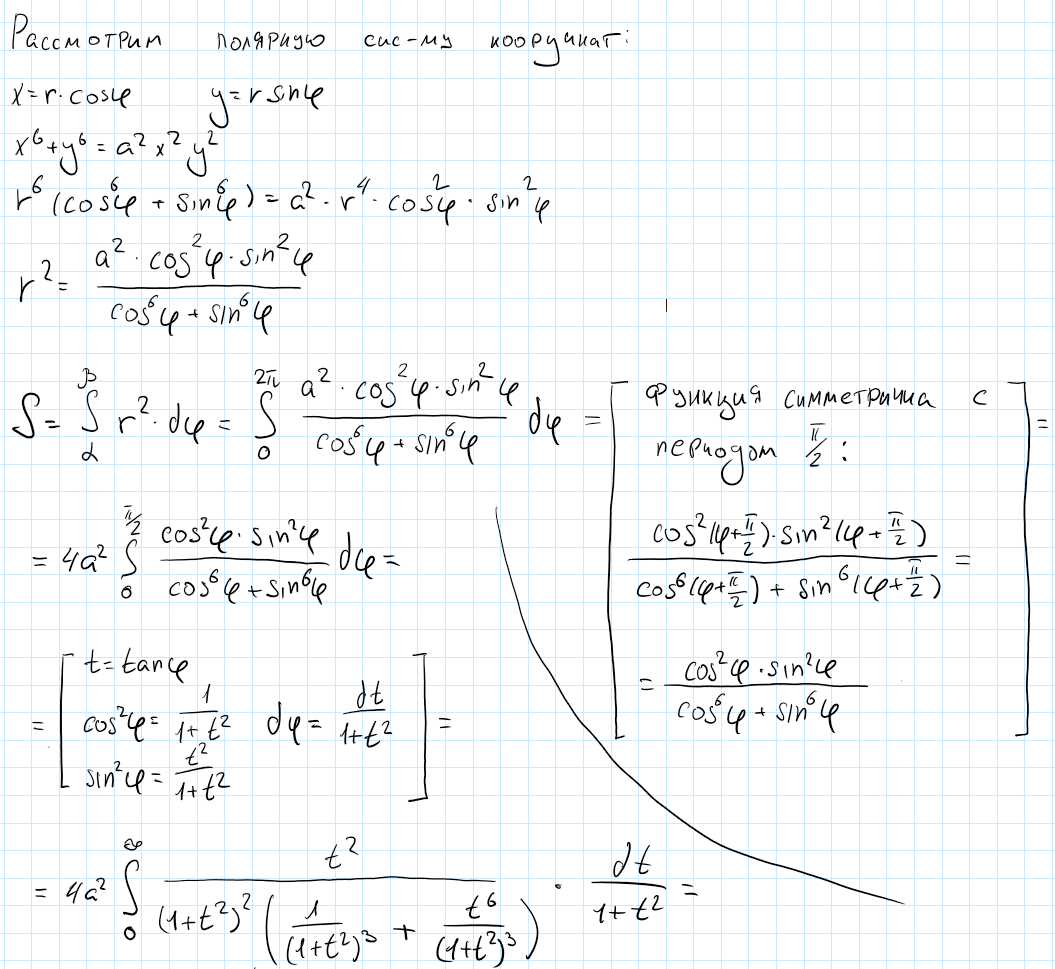
\includegraphics[width=\textwidth]{images/img41}
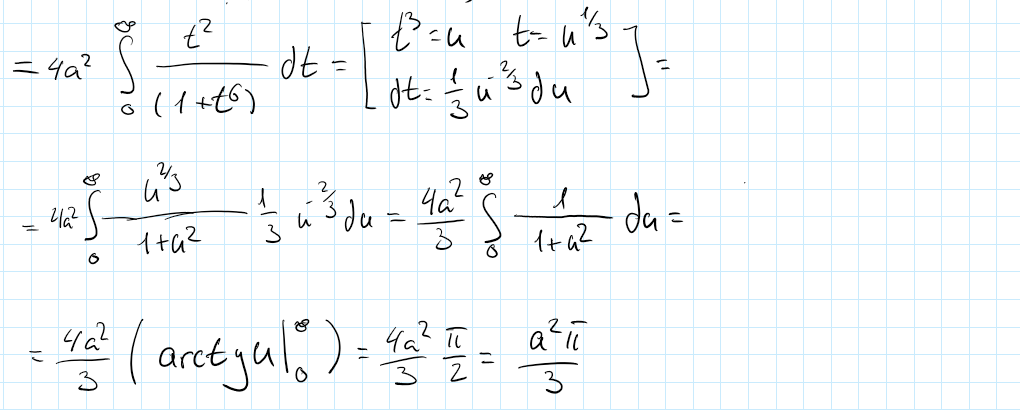
\includegraphics[width=\textwidth]{images/img42}
\newpage

\section*{Задание 5}
\textf{Найти длину кривой, заданной параметрически. Сделать рисунок.}
{\large
    \[
        x^2 + y^2 + z^2 = 9, |z| = y
    \]
}
\textbf{\Large Решение:\\}

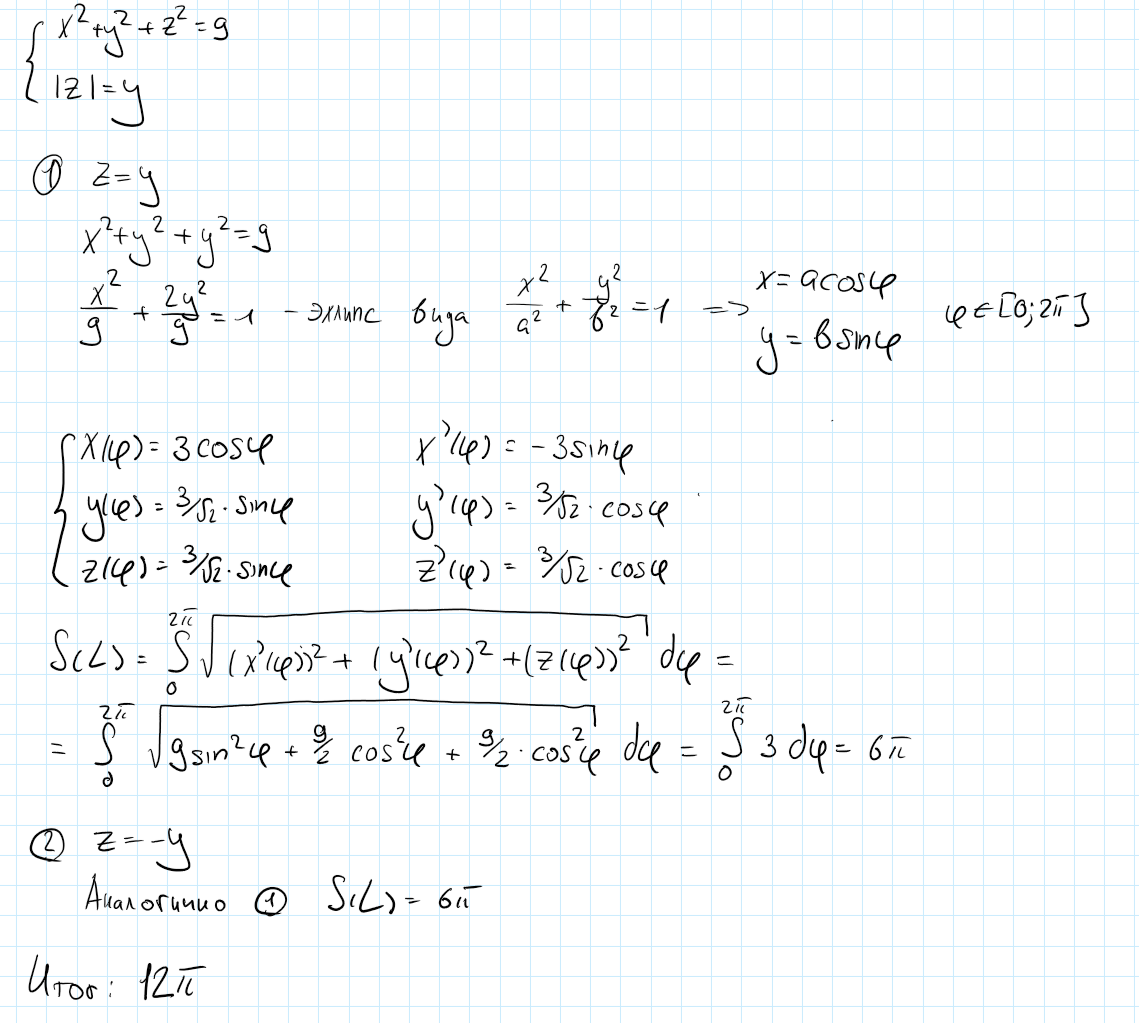
\includegraphics[width=\textwidth]{images/img51}
\newpage

\section*{Задание 6}
\textf{Исследовать интеграл на сходимость в каждой особой точке. Если функция меняет знак - на абсолютную и условную сходимость.}
{\large
    \[
        \int\limits_{1}^{\infty} \frac{\cos x}{x} \left( \frac{x + 1}{x} \right)^x \, dx
    \]
}
\textbf{\Large Решение:\\}

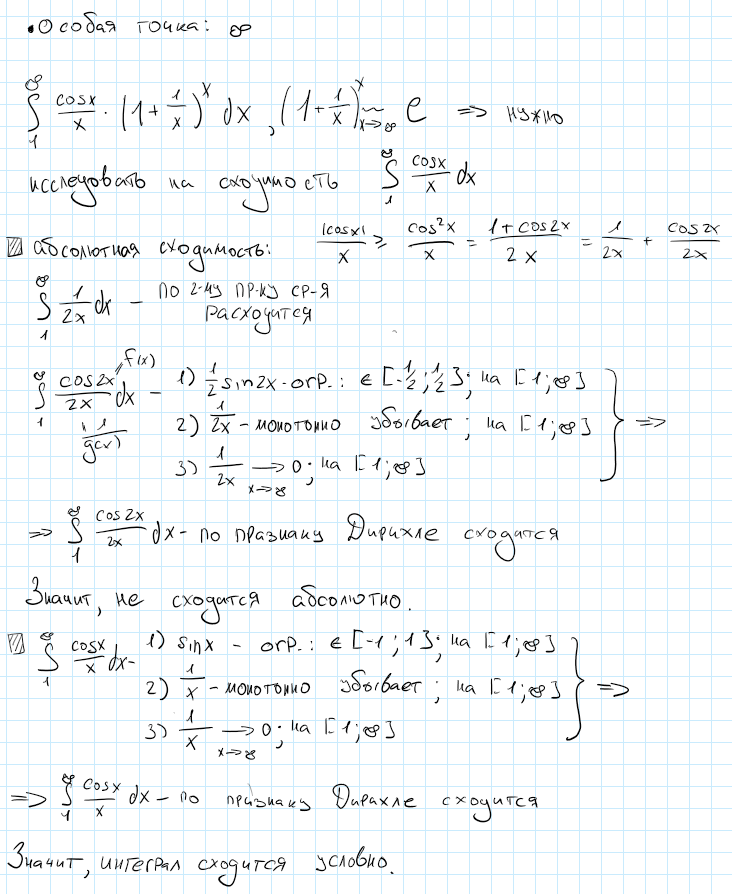
\includegraphics[width=\textwidth]{images/img61}
\newpage

\section*{Задание 7}
\textf{Исследовать интеграл на сходимость в каждой особой точке. Если функция меняет знак - на абсолютную и условную сходимость.}
{\large
    \[
        \int\limits_{0}^{\infty} \frac{\ln(1 + x + x^2) + \ln(1 - x + x^2)}{x^{3/2} (e^{x} + 1)} \, dx
    \]
}
\textbf{\Large Решение:\\}

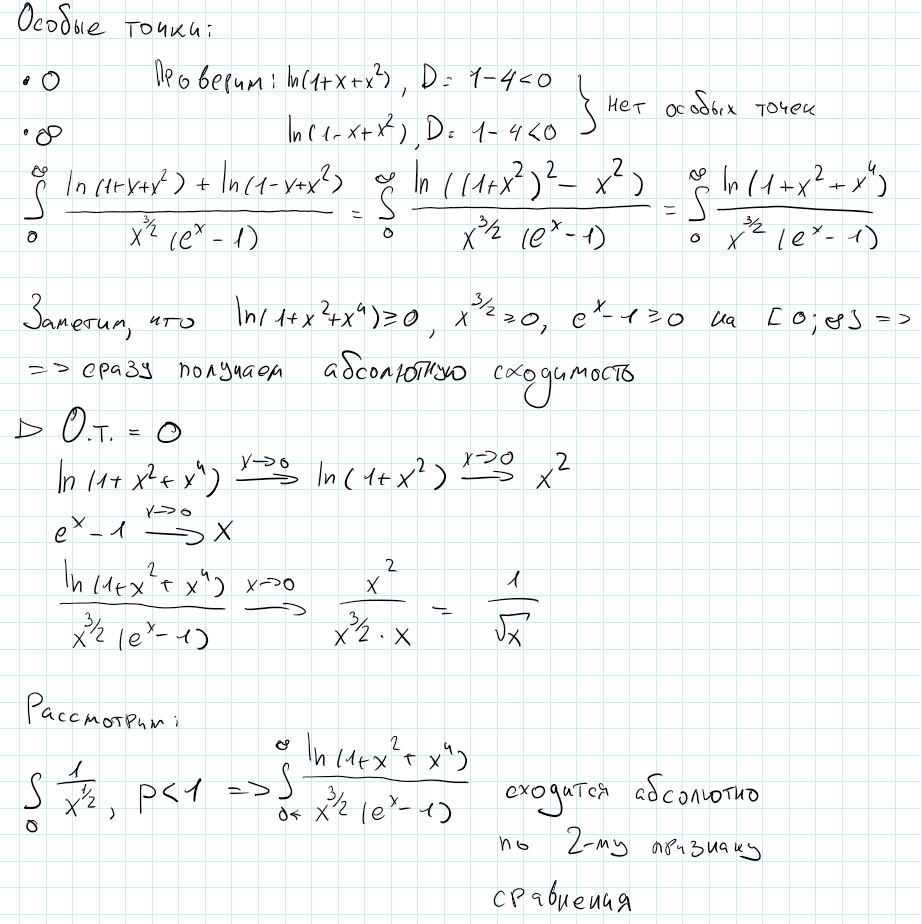
\includegraphics[width=\textwidth]{images/img71}
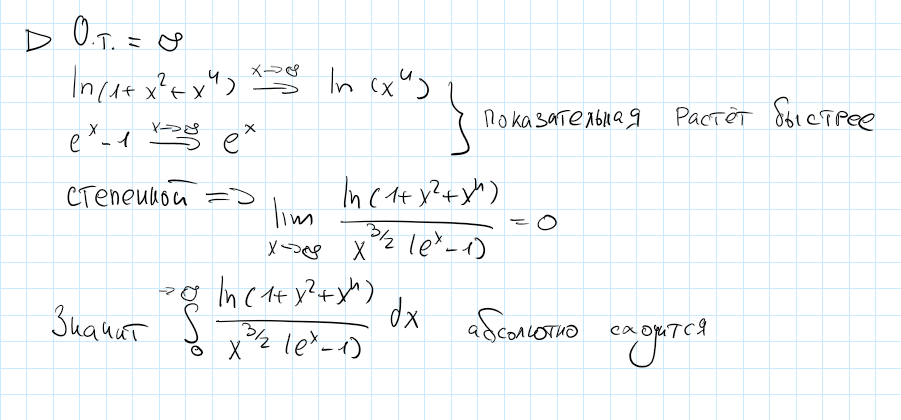
\includegraphics[width=\textwidth]{images/img72}
\newpage

\end{document}

